\documentclass{beamer}
\usetheme[secheader]{Madrid} % Themes without Navigation Bars
%\usetheme{PaloAlto} % Themes with a table of contents sidebar
%\usetheme{Copenhagen} % Themes with section and subsection tables

% Manage images
\usepackage{graphicx}
\graphicspath{ {./images/} }

% Custom commands
\newcommand{\highlight}[1]{{\color{blue} #1}}

% Title page and author information
\title{USpekPy Package}
\subtitle{Uncertainty estimation on protection quantities for x-rays using SpekPy and Monte Carlo techniques}
\author[X. Campo]{Xandra Campo}
\institute[LMRI-CIEMAT]{Ionizing Radiation Metrology Laboratory (LMRI) \newline CIEMAT, Spain}
\date{June 2024}

\begin{document}
	\maketitle
	
	\begin{frame}
		\frametitle{Table of Contents}
		\tableofcontents
	\end{frame}
	
	\section{Wellcome to USpekPy!}
	
	\begin{frame}
		\frametitle{Wellcome to USpekPy!}
		\tableofcontents[currentsection]
	\end{frame}
	
	\subsection{What is USpekPy?}
	
	\begin{frame}
		\frametitle{What is USpekPy?}
		\begin{itemize}
			\setlength\itemsep{1em}
			\item \highlight{Python package}: Open source and GPLv3-licensed library compatible with Python 3
			\href{https://github.com/lmri-met/uspekpy}{\beamergotobutton{Go}}
			\item \highlight{Goal}: Compute mean radiation protection quantities for a simulated x-ray spectrum with uncertainties using Monte Carlo techniques
			\item Based on \highlight{SpekPy}: Python package for modelling the x-ray spectra from x-ray tubes
			\href{https://bitbucket.org/spekpy/spekpy_release/wiki/Home}{\beamergotobutton{Go}}
		\end{itemize}
		\bigskip
		\centering
		\href{https://forms.gle/uCHj4XH5BJTBqjiQ9}{\beamergotobutton{Python usage poll}}		
	\end{frame}
	
	\subsection{Main features of USpekPy}
	
	\begin{frame}
		\frametitle{Main features of USpekPy}
		\begin{itemize}
			\setlength\itemsep{1em}
			\item Compute \highlight{mean values of radiation protection quantities} of a simulated x-ray spectrum: $\overline{E}$, $K_{air}$ and $\overline{h_K}$
			\item Compute \highlight{mean radiation protection quantities} of a simulated x-ray spectrum \highlight{with uncertainties} using Monte Carlo techniques: first and second HVL for Al and Cu, $\overline{E}$, $K_{air}$ and $\overline{h_K}$
			\item Perform \highlight{batch simulation} to compute mean values and uncertainties of radiation protection quantities for \highlight{several simulated x-ray spectra}
		\end{itemize}
	\end{frame}
	
	\subsection{USpekPy in a nutshell}
	
	\begin{frame}
		\frametitle{USpekPy in a nutshell}
		\begin{footnotesize}
			\begin{columns}
				\begin{column}{0.32\textwidth}
					\begin{exampleblock}{Status}
						\begin{tabular}{ll}
							Last version:&1.0.2\\
							Release date:&Jun 2024\\
							Maintenance:&Active\\
						\end{tabular}
					\end{exampleblock}
					\begin{block}{Testing}
						\begin{tabular}{ll}
							Tests:&Passing\\
							Code coverage:&65\%\\
						\end{tabular}
					\end{block}
					\begin{exampleblock}{Requirements}
						\begin{tabular}{ll}
							Python:&$\ge$3.8\\
							Dependencies:&spekpy\\
							&pandas\\
							&openpyxl\\
						\end{tabular}
					\end{exampleblock}
				\end{column}
				\begin{column}{0.55\textwidth}
					\begin{block}{Links}
						\begin{tabular}{lll}
							Source code:&GitHub&\href{https://github.com/lmri-met/uspekpy}{\beamergotobutton{Go}}\\
							Documentation:&README @GitHub&\href{https://github.com/lmri-met/uspekpy\#README}{\beamergotobutton{Go}}\\
							Contribute:&Issues @GitHub&\href{https://github.com/lmri-met/uspekpy/issues}{\beamergotobutton{Go}}\\
						\end{tabular}
					\end{block}
					\begin{exampleblock}{Authors}
						\begin{tabular}{ll}
							Authors:&X. Campo \& P. Avilés\\
							Email:&xandra.campo@ciemat.es\\
							&paz.aviles@ciemat.es\\
							Organization:&LMRI-Met @GitHub \href{https://github.com/lmri-met}{\beamergotobutton{Go}}\\
						\end{tabular}
					\end{exampleblock}
					\begin{block}{Distribution}
						\begin{tabular}{lll}
							Distribution:&PyPI&\href{https://pypi.org/project/uspekpy/}{\beamergotobutton{Go}}\\
							License:&GNU GPL v3.0&\href{https://github.com/lmri-met/uspekpy?tab=GPL-3.0-1-ov-file}{\beamergotobutton{Go}}\\
						\end{tabular}
					\end{block}
				\end{column}
			\end{columns}
		\end{footnotesize}
	\end{frame}
	
	\subsection{How to get support?}
	
	\begin{frame}
		\frametitle{How to get support?}
		\begin{columns}[t]
			\begin{column}{0.45\textwidth}
				\begin{block}{\centering Package documentation}
					\centering
					Check the \highlight{documentation} of USpekPy at GitHub
					\href{https://github.com/lmri-met/uspekpy\#readme}{\beamergotobutton{Go}}\\
					\medskip
					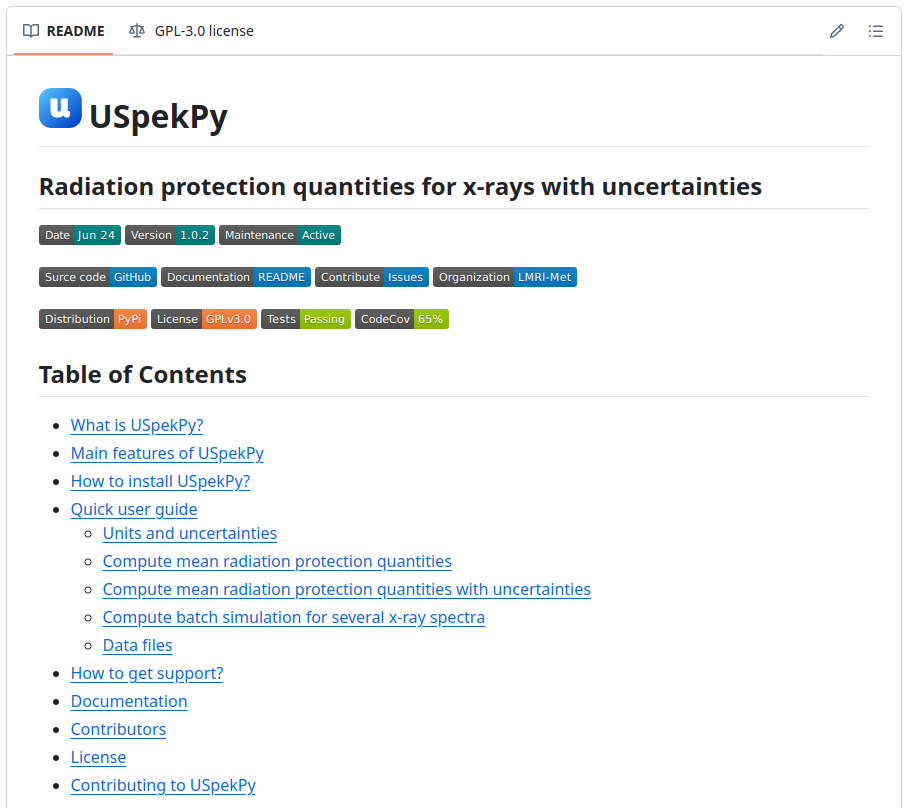
\includegraphics[width=\textwidth]{readme}
				\end{block}
			\end{column}
			\begin{column}{0.45\textwidth}
				\begin{block}{\centering Contact developers}
					\centering
					\bigskip
					Contact the developers of USpekPy \highlight{via email}:\\
					\bigskip
					Xandra Campo\\xandra.campo@ciemat.es\\
					\bigskip
					Paz Avilés\\paz.aviles@ciemat.es
				\end{block}	
			\end{column}
		\end{columns}
	\end{frame}
	
	\subsection{How to contribute to USpekPy?}
	
	\begin{frame}
		\frametitle{How to contribute to USpekPy?}
		\begin{columns}[t]
			\begin{column}{0.45\textwidth}
				\begin{block}{What may be a contribution?}
					\begin{itemize}
						\item Bug reports \& fixes
						\item Documentation improvements
						\item Feature enhancements
					\end{itemize}
				\end{block}
			\end{column}
			\begin{column}{0.45\textwidth}
				\begin{block}{How to deliver a contribution?}
					\begin{itemize}
						\item \highlight{Issues page} at GitHub (Recommended) \href{https://github.com/lmri-met/uspekpy/issues}{\beamergotobutton{Go}}
						\item Contact the developers \highlight{via email}
					\end{itemize}
				\end{block}	
			\end{column}
		\end{columns}
		\bigskip
		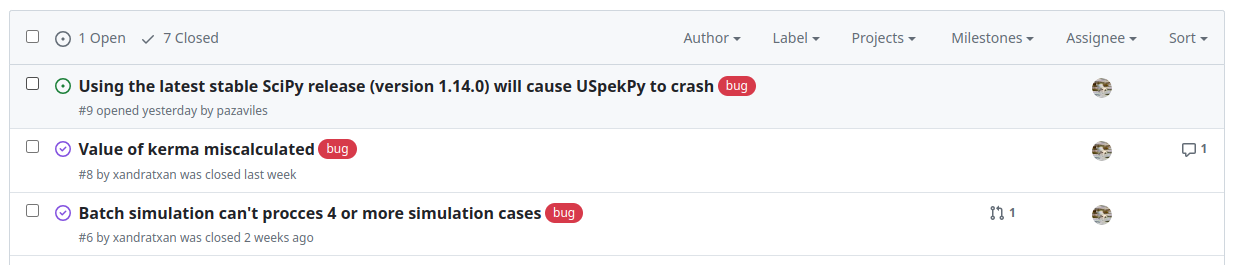
\includegraphics[width=\textwidth]{issues_list}
	\end{frame}
	
	\begin{frame}
		\frametitle{What to include in a contribution?}
		\begin{columns}
			\begin{column}{0.35\textwidth}
				\begin{itemize}
					\item Title
					\item Description
					\item Steps to reproduce
					\item Minimal, reproducible example
					\item Environment
					\item Error messages and logs
					\item Potential fix
				\end{itemize}
			\end{column}
			\begin{column}{0.65\textwidth}
				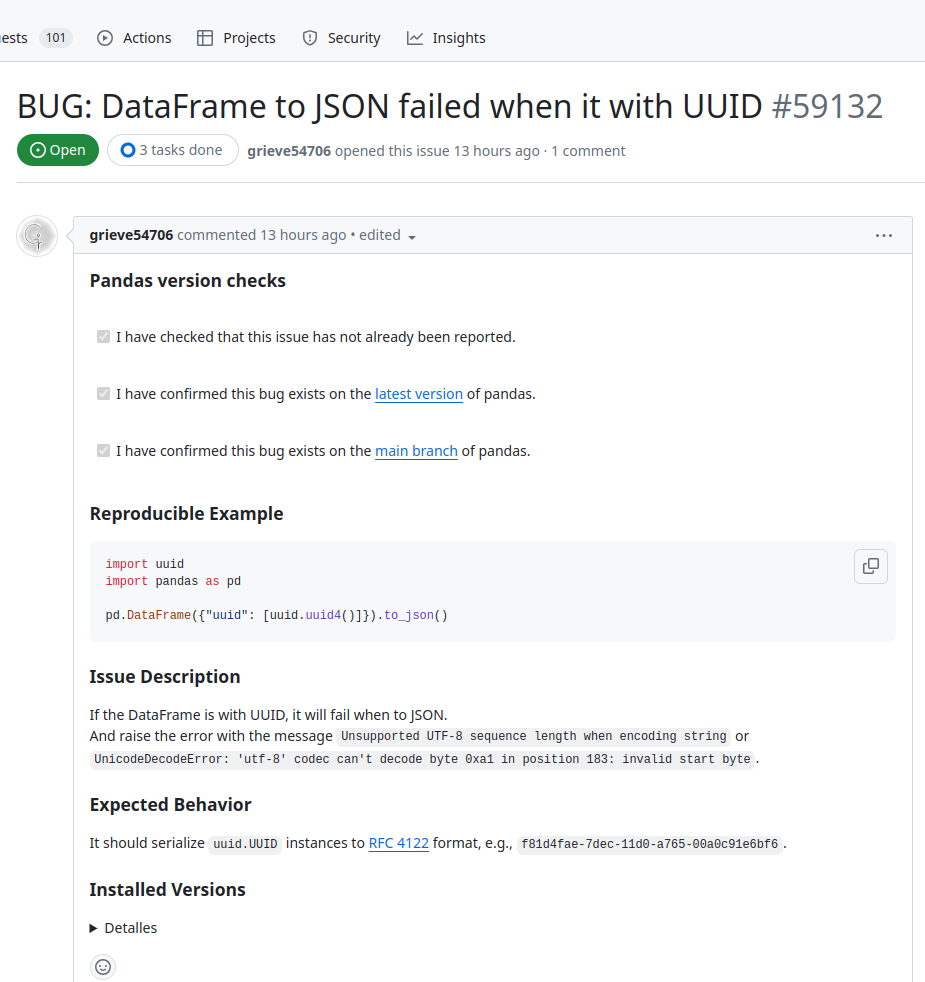
\includegraphics[width=\textwidth]{pandas_issue}
			\end{column}
		\end{columns}
	\end{frame}
	
	\section{Conclusion}
	
	\begin{frame}
		\frametitle{Conclusion}
		\tableofcontents[currentsection]
	\end{frame}
	
	\subsection{Improvements on the horizon}
	
	\begin{frame}
		\frametitle{Improvements on the horizon}
		\begin{itemize}
			\setlength\itemsep{1em}
			\item \highlight{Bug}: Fix SciPy dependency bug
			\item \highlight{New feature}: Add the contribution to the \highlight{uncertainty} of the variation of the mono-energetic air kerma-to-dose conversion coefficients
			\item \highlight{Documentation}: Improve package documentation (GitHub Wiki, GitHub Pages)
			\item \highlight{Testing}: Improve test code coverage
		\end{itemize}			
	\end{frame}
	
	\subsection{Let us know what you think}
	
	\begin{frame}
		\frametitle{Let us know what you think}
		\centering
		\highlight{Complete our satisfaction survey about this seminar!}
		
		Help us make future seminars better.
		
		\bigskip
		
		\href{https://forms.gle/zymzqsLidy5uxKQV6}{\beamergotobutton{Satisfaction survey}}
		
		\bigskip
		
		\highlight{Contribute to USpekPy package!}
		
		This sofware is for you. We want to make it fit better your necesities. Let us know if you find any issue or if you would like to have any new feature in future versions.
		
		\bigskip
		
		\href{https://github.com/lmri-met/uspekpy/issues}{\beamergotobutton{USpekPy Issues page}}
		
		xandra.campo@ciemat.es
		
		paz.aviles@ciemat.es
	\end{frame}
	
\end{document}
